 % TO DELETE

%    \documentclass[journal,a4paper]{IEEEtran}
\documentclass[journal]{IEEEtran}

%     \documentclass[10pt,twocolumn,twoside]{IEEEtran}
%     \documentclass[11pt,draftcls,onecolumn,peerreview]{IEEEtran} 
%         \topmargin       -6.0mm
%          \oddsidemargin      0mm
%          \evensidemargin     0mm
%          \textheight     223.5mm
%         \textwidth      170.0mm

\usepackage{color}
\newcommand{\mike}[1]{\textcolor{red}{#1}}
\newcommand{\dean}[1]{\textcolor{green}{#1}}
\newcommand{\parham}[1]{\textcolor{blue}{#1}} 
\newcommand{\ken}[1]{\textsf{\emph{\textbf{\textcolor{magenta}{#1}}}}} 
\newcommand{\cut}[1]{\textcolor{cyan}{#1}} 

\usepackage{cite}
%Reduce the spacing between figures and captions
% \usepackage[belowskip=-15pt,aboveskip=10pt]{caption}
%  \setlength{\intextsep}{2pt plus 2pt minus 2pt}

\ifCLASSINFOpdf
   \usepackage[pdftex]{graphicx}
  % declare the path(s) where your graphic files are
  % \graphicspath{{../pdf/}{../jpeg/}}
  % and their extensions so you won't have to specify these with
  % every instance of \includegraphics
  % \DeclareGraphicsExtensions{.pdf,.jpeg,.png}
\else
  % or other class option (dvipsone, dvipdf, if not using dvips). graphicx
  % will default to the driver specified in the system graphics.cfg if no
  % driver is specified.
  \usepackage[dvips]{graphicx}
  % declare the path(s) where your graphic files are
  % \graphicspath{{../eps/}}
  % and their extensions so you won't have to specify these with
  % every instance of \includegraphics
  % \DeclareGraphicsExtensions{.eps}
\fi

\usepackage[cmex10]{amsmath}
\interdisplaylinepenalty=2500
\usepackage{amssymb}
\ifCLASSOPTIONcompsoc
  \usepackage[tight,normalsize,sf,SF]{subfigure}
\else
  \usepackage[tight,footnotesize]{subfigure}
\fi


\usepackage{stfloats}
\usepackage{float}
\floatstyle{ruled}
\newfloat{algorithm}{htbp}{loa}%[chapter]
\floatname{algorithm}{Algorithm}

\begin{document}
%
% paper title
% can use linebreaks \\ within to get better formatting as desired
\title{Multi-Resolution Spatio-Temporal Neural Field Estimation }


\author{\parham{P. Aram}, \dean{D.R. Freestone~\IEEEmembership{Graduate Student Member,~IEEE}}, \mike{M. Dewar}, \ken{K.Scerri~\IEEEmembership{Member,~IEEE,}}, D.B. Grayden~\IEEEmembership{Member,~IEEE,} and V. Kadirkamanathan~\IEEEmembership{Member,~IEEE} % <-this % stops a space
\thanks{P. Aram* and V. Kadirkamanathan are with the Department of Automatic Control and Systems Engineering, University of Sheffield, Sheffield, S1 3JD, U.K. (e-mail:p.aram@sheffield.ac.uk; visakan@sheffield.ac.uk).}% <-this % stops a space
\thanks{D.\ R.\ Freestone and D.\ B.\ Grayden are with the Department
of Electrical and Electronic Engineering, The University of Melbourne, and The Bionic Ear Institute, VIC, Australia}
\thanks{M. Dewar is with the Department of Applied Physics and Applied Mathematics, Columbia University, New York, NY, USA}
\thanks{K. Scerri is with the Department of Systems and Control Engineering, University
of Malta, Msida, MSD 2080, Malta.}}
% <-this % stops a space
%\thanks{Manuscript received April 19, 2005; revised January 11, 2007.}}



% The paper headers
% \markboth{Journal of }%
% {Aram \MakeLowercase{\textit{et al.}}: Wavelet Multiresolution Spatio-Temporal Modelling Using the Integro-Difference Equation}
% The only time the second header will appear is for the odd numbered pages
% after the title page when using the twoside option.
% 
% *** Note that you probably will NOT want to include the author's ***
% *** name in the headers of peer review papers.                   ***
% You can use \ifCLASSOPTIONpeerreview for conditional compilation here if
% you desire.
 \ifCLASSOPTIONpeerreview
\else
\fi

% If you want to put a publisher's ID mark on the page you can do it like
% this:
%\IEEEpubid{0000--0000/00\$00.00~\copyright~2007 IEEE}
% Remember, if you use this you must call \IEEEpubidadjcol in the second
% column for its text to clear the IEEEpubid mark.

% make the title area
\maketitle


\begin{abstract}
%\boldmath
The Integro-difference equation (IDE) is an increasingly popular model of spatio-temporal processes. Here we develop a multi-resolution approximation (MRA) framework for the IDE neural field equations based on semi-orthogonal cardinal B-spline wavelets. State and parameter estimation is performed using the Expectation Maximization (EM) algorithm. A synthetic example is provided
to demonstrate the framework.
\end{abstract}
% Note that keywords are not normally used for peerreview papers.
% \begin{IEEEkeywords}
% Neural field model, multiresolution approximation (MRA), Expectation Maximization (EM) algorithm, wavelets.
% \end{IEEEkeywords}
% \IEEEpeerreviewmaketitle
\section{Introduction}
\IEEEPARstart{T}{he} human cerebral cortex has a multi-resolution architecture, where spatial scales for information processing range from ion channels, to single neurons, to networks of millions of neurons. This multi-resolution cortical architecture poses major modeling challenges to efficiently describe the brain's dynamics. This paper introduces a multi-resolution data-driven framework for neural field modeling, the Multi-Resolution Approximate Integro-Difference Equation (MRAIDE), to address this challenge. 

Neural field models describe the mass action of the central nervous system and are a critical link in our understanding of the biophysics of the EEG. These models typically describe the macroscopic dynamics of the human brain, but are also descriptive of finer-scale neurodynamics. The ability to create patient-specific neural models will contribute to our knowledge base of diseases such as epilepsy and will enable the development of new treatment strategies. This is particularly relevant to the advent of new devices that use therapeutic electrical stimulation. Stimulation strategies for devices currently operate in an open loop, where stimulation parameters are chosen using a process of trial and error. Therefore, there exists enormous potential to improve the performance of these devices using systems theory, which in turn requires a suitable dynamic model. Neural mass and neural field models are ideal candidates for estimation algorithms due to their strong links with physiology and their parsimony. It is expected that parameters of the neural fields models will be patient-specific and will, therefore, need to be inferred from data.

The first work describing data-driven mesoscopic neural modeling used a neural mass model to fit EEG data~\cite{Valdes1999}. This approach was extended to coupled neural masses through a Bayesian estimation scheme dubbed Dynamic Causal Modeling (DCM)~\cite{David2003}. Following this work, data-driven modeling was extended to continuum field equations that explained the richer dynamics of spatiotemporal neural fields \cite{Galka2008,schiff2008kalman,Daunizeau2009}. Most recently, a framework was developed where a finite element model (FEM) of the neural field (via a global Galerkin projection) was formed, using a basis function decomposition, to transform the PDE neural field equations into a finite dimension system to facilitate efficient state and parameter estimation~\cite{Freestone2011}. The current paper is an extension to this recent study, where we derive a neural field state-space model that accounts for the multi-resolution architecture and spatial dynamics of the human cortex. In this way, a flexible framework is created, whereby both macroscopic and microscopic behavior of the system can be represented simultaneously.

\section{IDE Neural Field Model}
The stochastic IDE form of the Amari neural field  formulation~\cite{Amari1977} is given by (see~\cite{Freestone2011} for a full derivation)
\begin{equation}\label{eq:DiscreteTimeModel}
	v_{t+1}\left(\mathbf{r}\right) = 
	\xi v_t\left(\mathbf{r}\right) + 
	T_s \int_\Omega { 
	    w\left(\mathbf{r},\mathbf{r'}\right)
	    f\left(v_t\left(\mathbf{r}'\right)\right) 
	\, d\mathbf{r}'} 
	+ e_t\left(\mathbf{r}\right), 
\end{equation}
where the post-synaptic membrane voltage at time $t$ of a population of neurons at position $\mathbf r$ is denoted $v_t\left(\mathbf r\right)$. Synaptic dynamics are included through the parameter $\xi=1-T_s/\tau$, where $\tau$ is the synaptic time constant and $T_s$ is the sampling time. The connectivity strength between neural populations at a distance $\mid\mathbf{r}-\mathbf{r'}\mid$ is described by the connectivity kernel $w\left(\mathbf{r}-\mathbf{r}'\right)$. The connectivity kernel is taken as a ``Mexican hat'' function, which describes local excitation and lateral inhibition \cite{Amari1977}. The term $e_t(\mathbf r)$ is an i.i.d. disturbance such that $e_t(\mathbf{s})\sim\mathcal{GP}(\mathbf 0,\eta(\mathbf{r}-\mathbf{r'}))$: a zero mean spatial Gaussian process with covariance function $\eta(\mathbf{r}-\mathbf{r'})$. The firing rate of the presynaptic neurons is related to the post-synaptic membrane potential by the activation function $f(v_t(\mathbf{r})) = \varsigma v_t(\mathbf{r})$ \cite{Murphy2009}.
%  due to high computational demands when using a nonlinear (sigmoidal) activation function. }
% \ken{Doing something just for computational efficiency only might be weak ... is there other work we can reference that makes the linearity assumption? ... or are there practical situations when this known to be a good approximations?} 
The observation equation describing the electrophysiological recordings is given by
\begin{equation}\label{eq:ObservationEquation}
	y_t(\mathbf{r}_{n_y}) = \int_{\Omega} { m\left(\mathbf{r}_{n_y}-\mathbf{r}'\right) v_t\left(\mathbf{r}'\right) \, d\mathbf{r}'} + \boldsymbol\epsilon_t(\mathbf{r}_{n_y}), 
\end{equation}
where $m\left(\mathbf{r}_{n_y}-\mathbf{r}'\right)$ is the observation kernel at location $\mathbf{r}_{n_y}$ and  $\boldsymbol{\epsilon}_{t}\sim \mathcal{N}\left(\mathbf{0},\mathbf{\Sigma}_{\epsilon}\right)$  is an i.i.d. Gaussian white noise process. % $\mathbf{y}_{t} = [y_t(\mathbf{r}_1) y_t(\mathbf{r}_2) \cdots y_t(\mathbf{r}_{n_y})]^\top$, compiled at $n_{y}$ spatial locations at time $t$ via the observation kernel , is corrupted by The superscript $\top$ denotes the transpose operator.
\section{MRA of the IDE in State-Space}
The multi-resolution approximation of the neural IDE (MRAIDE) is obtained by decomposing both the field, $v_t(.)$, and the connectivity kernel, $w(.)$, (assuming square-integrable functions) using translations and dilations of a scaling function $\phi(r)$ and a mother wavelet $\psi(r)$. Considering a one-dimensional field, the connectivity kernel is decomposed as,
\begin{equation}
 w\left(r-r'\right)=\sum_{l \in \mathbb{Z}}\alpha_{j_0,l}\phi_{j_0,l}\left(r-r'\right)+\sum_{j\geq j_0}^{\infty} \sum_{l \in \mathbb{Z}}\beta_{j,l}\psi_{j,l}\left(r-r'\right), 
\label{eq:KernelExpansion}
\end{equation}
where $\alpha_{j_0,l}$ are the approximation coefficients at the lowest scale $j_0$, and $\beta_{j,l}$ are the detail coefficients at different scales $j$, with $\phi_{j,l}\left(r\right)=2^{\frac{j}{2}}\phi\left(2^jr-l\right) $ and $\psi_{j,l}\left(r\right)=2^{\frac{j}{2}}\psi\left(2^jr-l\right)$. Integers $j$ and $l$ are the scale and translation parameters, respectively. Scaling functions retain the lowest frequency components, while the wavelet functions extract successively higher frequency components due to their low-pass and band-pass properties, respectively. The field is decomposed using
\begin{equation}
 v_t\left(r\right)=\sum_{l \in \mathbb{Z}}x_{t,j_{0},l}\phi_{j_{0},l}\left(r\right)+\sum_{j\geq j_0}^{\infty} \sum_{l \in \mathbb{Z}} \check{x}_{t,j,l}\psi_{j,l}\left(r\right),
\label{eq:FieldExpansion}
\end{equation}
where $x_{t,j_{0},l}$ and $\check{x}_{t,j,l} $ are the coefficients of the expansion and constitute the state vector at time $t$. %\dean{Need to define these guys as the states here!}

Equations \eqref{eq:KernelExpansion} and \eqref{eq:FieldExpansion} are infinite series expansions and must be truncated at some level $j$. The field and the connectivity kernel are approximated by
\begin{align}
	w\left(r-r'\right) &\approx \boldsymbol\theta^\top\boldsymbol\lambda\left(r-r'\right) 
	\label{eq:KernelFiniteExpansion} \\
	v_t\left(r\right) &\approx \boldsymbol\mu^\top\left(r\right)\mathbf{x}_t,
	\label{eq:FieldFiniteExpansion}
\end{align}
where the unknown parameter and state vectors, $\boldsymbol\theta \in \mathbb{R}^{n_{\theta}}$ and $\mathbf{x}_t \in \mathbb{R}^{n_x}$, are defined as 
\begin{align}
\boldsymbol\theta^\top &=[\begin{array}{ccccc} \boldsymbol\alpha_{j_0}^\top & \boldsymbol\beta_{j_0}^\top & \boldsymbol\beta_{j_0+1}^\top & \cdots & \boldsymbol\beta_{j}^\top \end{array}] 
\label{KernelWeights} \\
\mathbf{x}_{t}^\top &=[\begin{array}{ccccc}\mathbf{x}_{t,j_{0}}^\top &  \check{\mathbf{x}}_{t,j_{0}}^\top & \check{\mathbf{x}}_{t,j_{0}+1}^\top & \cdots & \check{\mathbf{x}}_{t,j}^\top\end{array}].
\label{FieldWeights}
\end{align}
The kernel and field approximation coefficient vectors, $\boldsymbol \alpha_{j_0}$ and $\mathbf{x}_{t,j_{0}}$, contain all the coefficients $\left\lbrace\alpha_{j_0, l}:l \in \mathbb{Z} \right\rbrace $ and $\left\lbrace x_{t,j_0, l}: l \in \mathbb{Z}\right\rbrace$, respectively. Similarly, the kernel and the field detail coefficient vectors, $\boldsymbol\beta_{j}$ and $\check{\mathbf{x}}_{t,j}$, contain all the coefficients $\left\lbrace \beta_{j,l} :l \in \mathbb{Z}\right\rbrace$ and $\left\lbrace  \check x_{t,j, l}:l \in \mathbb{Z}\right\rbrace$, respectively.

The vectors of the kernel and the field scaling and wavelet functions, $\boldsymbol\lambda$ and $\boldsymbol\mu$, respectively, are defined by
\begin{equation}
    \label{KernelBasisVector}
    \boldsymbol\lambda^\top(s)=[
    \boldsymbol\phi_{j_0}^\top(s) ~
    \boldsymbol\psi_{j_0}^\top(s) ~ 
    \boldsymbol\psi_{j_0+1}^\top(s) ~
    \cdots ~
    \boldsymbol\psi_{j}^\top(s)]
\end{equation} 
\begin{equation}
    \label{FieldBasisVector}
    \boldsymbol\mu^\top (r) = [
    \boldsymbol\phi_{j_0}^\top(r) ~ 
    \boldsymbol\psi_{j_0}^\top(r) ~ 
    \boldsymbol\psi_{j_0+1}^\top(r) ~ 
    \cdots ~ 
    \boldsymbol\psi_{j}^\top(r)
]   
\end{equation}


where $s=r-r'$. The vectors in  (\ref{KernelBasisVector}) and (\ref{FieldBasisVector}) are constructed in the same manner as the vectors in  (\ref{KernelWeights}) and (\ref{FieldWeights}). 
 
To derive the state-space model, we first define the matrices 
\begin{align}\label{eq:Lambdax}
 \mathbf{\Lambda}_{x} &\triangleq \int_{\Omega}\boldsymbol\mu\left(r\right)\boldsymbol\mu^\top\left(r\right) dr \\
\label{eq:Lambdatheta}
 \mathbf{\Lambda}_{\theta} &\triangleq \int_{\Omega}\boldsymbol\mu\left(r\right) \int_\Omega { 
	   \boldsymbol\theta^\top\boldsymbol\lambda\left(r-r'\right)
	    \boldsymbol\mu^\top\left(r\right)\ dr'dr.}
\end{align}
Substituting \eqref{eq:KernelFiniteExpansion} and \eqref{eq:FieldFiniteExpansion} in \eqref{eq:DiscreteTimeModel}, pre-multiplying by $\boldsymbol\mu\left(\mathbf r\right)$, and integrating over the space gives
\begin{align}\label{eq:DecomposedModel2} 
	&\mathbf{\Lambda}_{x} \mathbf{x}_{t+1}= 
	\xi\mathbf{\Lambda}_{x} \mathbf{x}_t +T_s \varsigma \mathbf{\Lambda}_{\theta}\mathbf{x}_t +\int_{\Omega}\boldsymbol\mu\left(r\right)e_t\left(r\right)dr.
\end{align}
Cross-multiplying by $\mathbf{\Lambda}_{x}^{-1}$ gives the state transition equation
\begin{align}\label{eq:StateEquation}
 \mathbf x_{t+1} &=\mathbf A(\boldsymbol \theta) \mathbf x_t+ \mathbf w_t\\
\label{eq:A_theta}
 \mathbf A(\boldsymbol \theta) &= T_s\varsigma\mathbf{\Lambda}_{x}^{-1}\mathbf{\Lambda}_{\theta}+\xi\mathbf I,
\end{align}
where $\mathbf I$ is the identity matrix. The disturbance becomes 
\begin{equation}\label{eq:Disturbance}
\mathbf w_t= \mathbf{\Lambda}_{x}^{-1}\int_{\Omega}\boldsymbol\mu \left(r\right)e_t\left(r\right)dr,
\end{equation}
which is a vector valued, zero-mean normally distributed, white noise process with covariance (see \cite{Freestone2011} for proof)
\begin{equation}
\boldsymbol\Sigma_w =\mathbf{\Lambda}_{x}^{-1}\iint\limits_{\boldsymbol\Omega}\boldsymbol\mu\left(r\right) \eta\left(r-r'\right)\boldsymbol\mu^{\top}\left(r'\right)dr'dr\mathbf{\Lambda}_{x}^{-\top}.
\end{equation}
The observation equation of the state-space model is found by substituting decomposition \eqref{eq:FieldFiniteExpansion}
 into \eqref{eq:ObservationEquation} giving
\begin{equation}\label{eq:ReducedObservationEquation} 
	\mathbf{y}_t = \mathbf{C}\mathbf{x}_t + \boldsymbol{\varepsilon}_t,
\end{equation}
where each element of the observation matrix is given by
\begin{equation}\label{eq:Observationmatrix}
	\mathbf{C}_{ij} \triangleq \int_{\Omega}m(r_i - r')\boldsymbol{\mu}_j(r') \, d\mathbf{r}'.
\end{equation}

The MRAIDE can be implemented using various scaling and wavelet functions. B-spline functions were chosen due to their compact support and the ability to analytically define the convolution and inner product to form $\boldsymbol\Lambda_x$ and $\boldsymbol \Lambda_{\theta}$. To show how $\boldsymbol\Lambda_x$ and $\boldsymbol \Lambda_{\theta}$ are formed, the $m^{th}$ order cardinal B-spline scaling function is defined by the recurrence relation \cite{Chui1992} 
\begin{equation}
N_{m}\left(r\right) = \left(N_{m-1}\ast N_{1}\right)\left(r\right) = \int_0^{1} N_{m-1}\left( r-r'\right)dr',
\label{SplineConvolutionIntegral}
\end{equation}
where $m>1$, $\ast$ denotes convolution, and $N_1\left(r\right)$ is the characteristic function of the unit interval $\left[ 0,1\right)$.
% \begin{equation}
% N_{1}\left(r\right)=
% \begin{cases}
% 1 & \text{if $ 0\le r<1$}, \\
% 0 & \mathrm{elsewhere}.
% \end{cases}
% \end{equation}
Equation \eqref{SplineConvolutionIntegral} can be rewritten as $(m-1)$ convolutions of the indicator function with itself since
\begin{equation}
 N_{m}\left(r\right)=\underbrace{\left(N_{1}\ast N_{1}\ast \cdots \ast N_{1}\right)}_{m-1\quad \text{convolutions}}\left(r\right).
\end{equation}
Using the associativity property of convolution, we have
\setlength{\arraycolsep}{0.0em}
\begin{align}\label{eq:BsplineConvolution}
N_{m}\left( r\right) \ast N_{m'}\left(r\right)&=\underbrace{\overbrace{\left(N_{1} \ast \cdots \ast N_{1}\right)}^{m-1 \quad \text{convolutions}}\left(r\right) \ast \overbrace{\left(N_{1} \ast \cdots \ast N_{1}\right)}^{m'-1\quad \text{convolutions}}}_{m+m'-1 \quad \text{convolutions}}\left(r\right)\nonumber\\
&=N_{m+m'}\left(r\right).
\end{align}
A direct consequence of \eqref{eq:BsplineConvolution} is the inner product between two B-splines is another translated B-spline such that
\begin{align}
 \left\langle N_{m}\left(r-l_{1}\right), N_{m'}\left(r-l_{2}\right)\right\rangle=&N_{m+m'}\left(m+l_{1}-l_{2}\right)\nonumber \\
=&N_{m+m'}\left(m'+l_{2}-l_{1}\right),
\label{eq:BsplineInnerProduct}
\end{align}
where $\left\langle \cdot,\cdot\right\rangle $ denotes the inner product. This holds as the support of $N_m\left(r\right)$ is $\left[ 0,m\right]$ and  is symmetric with respect to $r=\frac{m}{2}$. The $m^{th}$-order B-spline wavelet is defined as \cite{Chui1992}
\begin{align}
 \varphi & _{m}\left(r\right) = \sum_{n=0}^{3m-2} \frac{\left(-1\right)^n}{2^{m-1}}  q_n N_{m}\left(2r-n\right) \\
 q & _n = \sum_{l=0}^{m} \binom{m}{l} N_{2m}\left(n-l+1\right), \,  \text{ $0\le n\le 3m-2$},
\end{align}
where $q_n$ are the coefficients. By exploiting \eqref{eq:BsplineConvolution} and \eqref{eq:BsplineInnerProduct}, the integrals in \eqref{eq:Lambdax} and \eqref{eq:Lambdatheta} can be computed analytically. In order to calculate elements of $\boldsymbol\Lambda_{x}$ and $\boldsymbol\Lambda_{\theta}$, the scaling and wavelet basis functions must be expanded in terms of $N_m$ at the appropriate scale. In this paper, $4^{th}$ order cardinal B-spline scaling and wavelet functions are used. Therefore, the $8^{th}$ and $12^{th}$ order B-spline values at integer points are required (see \cite{Goswami1999}) to compute the integrals in \eqref{eq:Lambdax} and \eqref{eq:Lambdatheta}.
\section{State and Parameter Estimation}
The state-space representation of the MRAIDE allows the use of the well known Expectation Maximization (EM) algorithm \cite{Dempster1977} to infer both the kernel and the field from electrophysiological data. The EM algorithm, when used in this context \cite{Dewar2009}, yields the maximum likelihood kernel estimate and the posterior distribution of the field over time. We use the standard EM algorithm for linear dynamic systems \cite{Roweis1999,Shumway2000} and hence only describe aspects of the algorithm that are specific to MRA neural field equations. EM essentially finds increasingly tighter lower bounds on the likelihood of the kernel $p(\mathbf{y}_1 \ldots \mathbf{y}_T|w)$ so that, at convergence, the maximum of the bound corresponds to the maximum of the likelihood. For the linear state-space model given by (\ref{eq:StateEquation}-\ref{eq:Observationmatrix}), the bound used is a quadratic of the form
\begin{equation}\label{eq:Qfunction}
 \mathcal Q\left(\boldsymbol \theta,\boldsymbol\theta'\right)=\beta+2T_s\varsigma\left(\boldsymbol\upsilon_0-\boldsymbol\upsilon_1\right)\boldsymbol\theta-T_s\varsigma\boldsymbol\theta^\top\boldsymbol\Upsilon\boldsymbol\theta,
\end{equation}
where $\beta$ is constant with respect to $\boldsymbol\theta$. Equation \eqref{eq:Qfunction} is maximum at $\boldsymbol \theta= \boldsymbol\Upsilon^{-\top}(\boldsymbol\upsilon_0^\top-\boldsymbol\upsilon_1^\top)$, where
% \begin{align}
%  \boldsymbol \theta= \boldsymbol\Upsilon^{-\top}(\boldsymbol\upsilon_0^\top-\boldsymbol\upsilon_1^\top),
% \end{align}
% where
\begin{align}\label{eq:upsilon0}
 \boldsymbol\upsilon_0 & =\sum_{i,j=1}^{n_x}[\boldsymbol\Xi_0]_{i,j}[\boldsymbol\Gamma_1]^{j,i} \\ 
 \boldsymbol\upsilon_1 & =\xi\sum_{i,j=1}^{n_x}[\boldsymbol\Xi_1]_{i,j}[\boldsymbol\Gamma_2]^{j,i} \label{eq:upsilon1}\\
 \boldsymbol\Upsilon&=T_s\varsigma\sum_{i,j=1}^{n_x}[\boldsymbol\Xi_1]_{i,j}[\boldsymbol\Gamma_3]^{j,i},\label{eq:Upsilon}
\end{align}
where $[.]_{p,q}$ denotes the $\left(p,q\right)$-element of the matrix, and $ [.]^{p,q}$ denotes the $\left(p,q\right)$-block of the block matrix, and where
\begin{align}
 [\boldsymbol\Gamma_1]^{j,i} & =\sum_{k=1}^{n_x}[\boldsymbol\Sigma_{w}^{-1}\boldsymbol\Lambda_{x}^{-1}]_{j,k}[\mathbf U]^{k,i}\label{eq:Gamma1} \\ 
 [\boldsymbol\Gamma_2]^{j,i} & =\sum_{k=1}^{n_x}[\boldsymbol\Sigma_{w}^{-1}\boldsymbol\Lambda_{x}^{-1}]_{j,k}[\mathbf U]^{k,i}\label{eq:Gamma2} \\
[\boldsymbol\Gamma_3]^{j,i}&=\sum_{k,m=1}^{n_x}[\mathbf{U}^{\top}]^{j,m}[ \boldsymbol\Lambda_{x}^{-1}\boldsymbol\Sigma_{w}^{-1}\boldsymbol\Lambda_{x}^{-1}]_{m,k}[\mathbf{U}]^{k,i}\label{eq:Gamma3}.
\end{align}
Each $1\times n_{\theta}$ block of the $n_x \times n_x n_{\theta}$ block matrix $\mathbf U$ is
\begin{align}
\left[ \mathbf U\right] ^{i,j}&=\int_{\boldsymbol \Omega}\left[\boldsymbol\mu(r) \right]_i \left[\int_{\boldsymbol\Omega} \boldsymbol\mu\left(r'\right)\boldsymbol \lambda^\top \left(r-r'\right) dr'\right]_{j:} dr,
\end{align}
where $[.]_{j:} $ denotes the $j^{th}$ row. All $n_x^2$ blocks of $\boldsymbol\Gamma_1$,$\boldsymbol\Gamma_2$, and $\boldsymbol\Gamma_3$  can be computed before the commencement of the EM iterations. Note that to separate $\boldsymbol\theta$ from $\boldsymbol\Lambda_{\theta}$ in forming the $\mathcal{Q}$-function we used the relation
\begin{equation}
\left[ \boldsymbol\Lambda_{\theta}\right] _{i,j} =\left[ \mathbf U\right]^{i,j}\boldsymbol\theta. 
\end{equation}

The matrices $\boldsymbol\Xi_0$ and $\boldsymbol\Xi_1$ are calculated using the Rauch Tung Streibel smoother \cite{RAUCH1965} outputs: state estimates, $\hat{\mathbf x}_t$, covariance, $\mathbf P_t=\mathrm{cov}(\mathbf{x_t})$, and cross-covariance matrix, $\mathbf M_t=\mathrm{cov}(\mathbf{x}_{t-1},\mathbf{x}_{t})$ \cite{Gibsona2005},
\begin{align}\label{eq:Xivariables}
\boldsymbol\Xi_0&=\sum_{t=0}^{T-1}\left(\mathbf M_{t+1}+\mathbf{\hat x}_t\mathbf{\hat x}_{t+1}^\top\right) \\
 \boldsymbol\Xi_1&=\sum_{t=0}^{T-1}\left(\mathbf P_t+\mathbf{\hat x}_t\mathbf{\hat x}_t^\top\right).
\end{align}
The algorithm has two steps: the E-step, which computes $\boldsymbol\Xi_0$ and $\boldsymbol\Xi_1$ based on the most recent parameter estimates using the RTS smoother, and the M-step, which updates the parameter estimates by computing the (analytic) maximum of $Q(\theta,\theta')$. The EM algorithm iterates between these two steps until the parameter estimates converge.
%\cut{The second terms in  \eqref{eq:upsilon0}, \eqref{eq:upsilon1}, and \eqref{eq:Upsilon} can be computed as a once-off before the commencement of the EM iterations, which increases the speed of the M-step significantly compared to the method in \cite{Dewar2009}.}

\section{Results}
To demonstrate the performance of the MRAIDE estimation framework, data was generated synthetically  using \eqref{eq:DiscreteTimeModel} and \eqref{eq:ObservationEquation}, enabling a comparison between true and estimated parameters. 200 realizations of 1~s of data were generated, where the estimation was applied to the final 900~ms, allowing the model's initial transients to die out. The observation noise was set to $\boldsymbol\Sigma_{\epsilon}=0.1 \times \mathbf{I}_{n_y}$ and the disturbance covariance was set to $\eta(r-r') = \phi_{3,-2}(r-r')$ (B-spline, $j=3$). The sampling period and the synaptic time constant were set to $T_s = 1$~ms and $\tau = 10$~ms, respectively. The firing rate slop, $\varsigma$ was set to $0.56~mV^{-1}$. The distance between adjacent sensors was $0.5$~mm, resulting into $n_y = 161$ observations. The observation kernel was modeled using a B-spline function, with a width of 0.8~mm at half the maximum amplitude. The spacing and bandwidth of the sensors allowed for the full spatial bandwidth of the field to be observed.  %\ken{if we need to gain space I would remove the rest of this paragraph and put all parameters in a table} 
The spatial cutoff frequency of the observed field was used to specify the level of decomposition required to represent the field using the wavelets. Using an oversampling parameter of 5, the cutoff spatial frequency was $\nu_{cy} \approx 6.9 $ cycles/mm, \parham{this was obtained by averaging the spectral power of the spatial frequency (over time) from the observations} \cite{Scerri2009}. Therefore, wavelets up to level $j=3$ (with the bandwidth $\approx[5,8]$ cycles/mm) can represent the significant spatial characteristics of the field, yielding $n_x = 131$ states. 

% \dean{With this number of observations, the estimation problem was well-posed, since the wavelets are orthogonal and the number of states, $n_x < n_y$ at each level of the decomposition.}  
% \cut{Note that wavelets due to their bandpass filter characteristics extract successively higher and higher frequency components by increasing $j$.}

The field reconstruction, at different levels of approximations, is shown in \figurename{\ref{fig:FieldEstimates}}. The figure confirms that $j=3$ is adequate to capture the dynamics of the underlying field, where the RMSE converges to a steady value of 0.78. Fig.~\ref{fig:FieldEstimates} confirms good state estimation performance, where the estimated field is in good accordance with the true field. 

The actual connectivity kernel and the decomposition is plotted in \figurename{\ref{fig:KernelEstimate}}(a). No assumptions where made about the shape of the kernel. The reconstructed kernel is in good accordance with the actual kernel, where the actual kernel lies inside the confidence interval. \parham{Large standard deviation is due to the high number of parameters.} The small error in the estimate is attributed to the MRA of the system used to form the estimator. \figurename{\ref{fig:KernelEstimate}}(b) and (c) shows the kernel scaling and wavelet functions, respectively.
\begin{figure}[!h] 
	\centering
		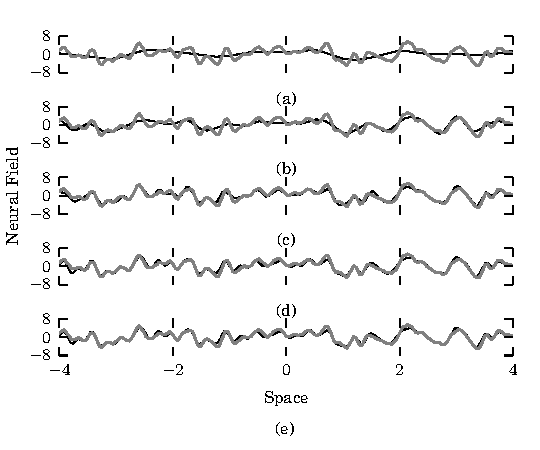
\includegraphics[scale=1]{./Graph/fig1.pdf}
		\caption{Actual (gray) and estimated (black) neural fields at a time instant for different spatial resolutions. (a) $j=0$, $n_x=17$, $RMSE = 1.93$. (b) $j=1$, $n_x=33$, $RMSE = 1.39$. (c) $j=2$, $n_x=65$, $RMSE = 0.90$. (d) $j=3$, $n_x=131$, $RMSE = 0.78$. (e) $j=4$, $n_x=263$, $RMSE=0.78$.}
	\label{fig:FieldEstimates}
\end{figure} 
\begin{figure}[!h] 
	\centering
		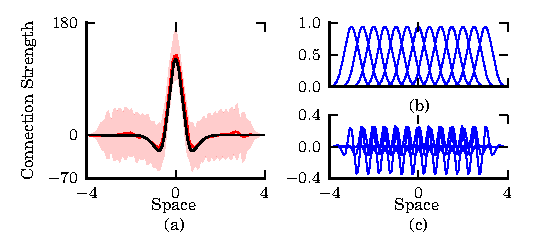
\includegraphics[scale=1]{./Graph/fig2.pdf}
		\caption{Connectivity kernel estimate. (a) The actual kernel is shown with the black solid line. The mean kernel estimates over 200 realizations and confidence interval are shown by the red line and red shaded region ($\pm2$ std.). (b)-(c) Kernel scaling and wavelets functions, respectively, at $j=1$.}
	\label{fig:KernelEstimate}
\end{figure}
% \caption{The actual connectivity kernel is shown with the black solid line. The estimated kernel and confidence interval is shown by the red line and red shaded region ($\pm2$ std.). The 7 weighted kernel basis functions are shown by the black dashed lines.}
\section{Discussion}
In this paper, we have presented a novel model-based framework for estimating cortical dynamics from electrophysiological measurements. The novel and key developments of the paper include the multi-resolution FEM representation of the neural field, and the estimator for an intracortical connectivity kernel with an arbitrary shape. This work is significant, as the ability to create patient specific neural field models has the potential to contribute to our understanding and improve treatment of diseases resulting from abnormal neurodynamics, such as epilepsy. Other groups have previously highlighted the importance of a multi-resolution approach in neural field modeling. For example, it is thought that the dynamics and connectivity structure differs at different spatial scales~\cite{Qubbaj2009}.

The MRAIDE approach is not limited to neural fields; the framework can be applied to modeling other multi-resolution spatiotemporal dynamical systems such as weather systems, ecological systems, and others\cite{Wikle2002,Xu2005,Fort2008}. 
% \ken{meteorology [76, 88, 94, 222, 232], epidemiology [123, 137, 218], physics [32, 85, 129, 231], environmental science [45, 87, 183, 204] and economics [31, 48, 165]. (This is copy and paste from my thesis ... parham I'll get you the references later)}. \parham{Mike,Ken: can add to this list?}\mike{While I love this kind of thing for a review, I'm not sure we have space for this kind of thing? Also it's not terribly specific. I think it's better to stick to how it has the potential to model brains in a manner that rocks, rather than loosely saying it could be applied to any spatiotemporal system, i.e. literally everything.}

  \mike{The framework makes two key assumptions about the cortex: a linear activation function and stationary dynamics. Our main aim for this framework in the future is to relax these assumptions using the multi-resolution decomposition. While the decomposition itself holds, efficiently performing nonlinear smoothing in the much larger state space remains a challenge. Additional avenues for future work include extending the model to capture a second order synaptic response kernel, and time delays \parham{at lower spatial resolutions}.  The estimation techniques should also be extended to deal with spatial and temporal heterogeneity in the kernel. Finally, the majority of our current work involves applying this framework to collected data, primarily for the use of seizure detection and mitigation.}

 In order to apply the framework to real data some assumptions must be made, such as stationarity of the parameters over the estimation period. Perhaps the most critical assumption is that the model provides an apt description of the cortical dynamics. The authors acknowledge that there is, and will always be, a discrepancy between the model and cortex. Nevertheless, the model-based framework proposed in this paper may enable meaningful state tracking and connectivity estimation. The key development in this paper is the multi-resolution decomposition forming the state-space model \parham{and its ability to approximate the neural field at required resolution.} \cut{The decomposition holds for more sophisticated nonlinear forms of the field equations, where the unscented RTS smoother should be used in the E-step of the estimation algorithm.}

% \cut{Future work should be directed towards extending the framework to account for a second-order synaptic response kernel, heterogeneity in the connectivity and perhaps time delays at lower spatial resolutions. Most importantly, future work should be directed towards applying and validating the framework on real data.}

% use section* for acknowledgement
%\section*{Acknowledgment}

% Can use something like this to put references on a page
% by themselves when using endfloat and the captionsoff option.
\ifCLASSOPTIONcaptionsoff
  \newpage
\fi

%   \newpage
% \bibliographystyle{unsrt} 
% \bibliography{MRAIDE}

\bibliographystyle{IEEEtran}
% argument is your BibTeX string definitions and bibliography database(s)
 \bibliography{IEEEabrv,MRAIDE}


\end{document}


